\documentclass[12pt, twoside]{article}
\usepackage[letterpaper, margin=1in, headsep=0.5in]{geometry}
\usepackage[english]{babel}
\usepackage[utf8]{inputenc}
\usepackage{amsmath}
\usepackage{amsfonts}
\usepackage{amssymb}
\usepackage{tikz}
\usetikzlibrary{quotes, angles}
\usepackage{graphicx}
\usepackage{enumitem}
\usepackage{multicol}

\newif\ifmeta
\metatrue %print standards and topics tags

\title{Regents Geometry}
\author{Chris Huson}
\date{October 2021}

\usepackage{fancyhdr}
\pagestyle{fancy}
\fancyhf{}
\renewcommand{\headrulewidth}{0pt} % disable the underline of the header
\raggedbottom


\fancyhead[LE]{\thepage}
\fancyhead[RO]{\thepage \\ Name: \hspace{4cm} \,\\}
\fancyhead[LO]{BECA / Dr. Huson / Geometry 03 Parallels and transversals}

\begin{document}

\subsubsection*{3.4 Transversals and review}
\begin{enumerate}
  \item Do Now: Given $\overline{DEFG}$, $DE=3 \frac{1}{4}$, $EF=6 \frac{1}{4}$, and $FG= 1 \frac{3}{4}$. (diagram not to scale)\\ [0.25cm]
  Find ${DG}$, expressed as a fraction, not a decimal. \vspace{1cm}
  \begin{flushleft}
      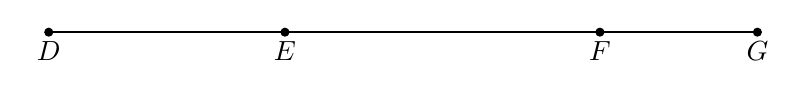
\begin{tikzpicture}
        \draw [-, thick] (0,0)--(9,0);
        \draw [fill] (0,0) circle [radius=0.05] node[below]{$D$};
        \draw [fill] (3,0) circle [radius=0.05] node[below]{$E$};
        \draw [fill] (7,0) circle [radius=0.05] node[below]{$F$};
        \draw [fill] (9,0) circle [radius=0.05] node[below]{$G$};
      \end{tikzpicture}
    \end{flushleft}


\item Do Now: Given $P(-2.4)$ and $Q(1.8)$, as shown on the number line. 
  Find the length of the line segment $\overline{PQ}$. 
  \begin{flushright}
    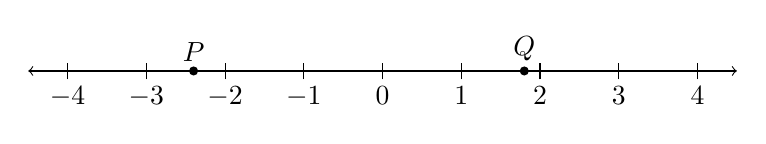
\begin{tikzpicture}
      \draw [<->] (-4.5,0)--(4.5,0);
      \draw [-, thick] (-2.4,0)--(1.8,0);
      \foreach \x in {-4,...,4} %2 leading for diff!=1
        \draw[shift={(\x,0)},color=black] (0pt,-3pt) -- (0pt,3pt) node[below=5pt]  {$\x$};
        \draw [fill] (-2.4,0) circle [radius=0.05] node[above] {$P$};
        \draw [fill] (1.8,0) circle [radius=0.05] node[above] {$Q$};
    \end{tikzpicture}
  \end{flushright} \vspace{1cm}

\item Spicy Do Now: Solve for $x$, $x^2+10x+7=2x$ \vspace{6cm}

\item Given two parallel lines and a transversal, as shown, with $m\angle 6 =  68^\circ$. Write down the value of each angle measure.
  \begin{multicols}{2}
    \begin{enumerate}[itemsep=0.5cm]
      \item What angle is corresponding to $\angle 6$?
      \item What angle is alternate interior to $\angle 4$?
      \item Find $m\angle 1$
    \end{enumerate}
    \begin{flushright}
      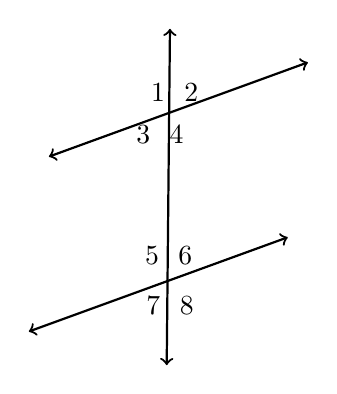
\begin{tikzpicture}[scale=1,rotate=20]
      \draw [<->, thick] (3.5,2)--(7,2);
      \draw [<->, thick] (2.5,0)--(6,0);
      \draw [<->, thick] (4,-1)--(5.5,3);
      \node at (4.5,0.3) [left]{$5$};
      \node at (4.5,0.3) [right]{$6$};
      \node at (4.3,-0.3) [left]{$7$};
      \node at (4.3,-0.3) [right]{$8$};
      \node at (5.2,2) [above left]{$1$};
      \node at (5.2,2) [above right]{$2$};
      \node at (5,2) [below left]{$3$};
      \node at (5,2) [below right]{$4$};
    \end{tikzpicture}
  \end{flushright}
  \end{multicols}

\newpage
  \item Given two parallel lines and a transversal, with $m\angle 3 = 18(x-1)$ and $m\angle 5 = 18(x+1)$. Find $m\angle 1$. (First write an equation, and solve for $x$)
\begin{flushright}
  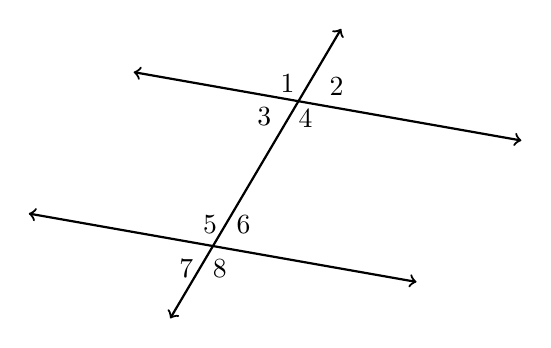
\begin{tikzpicture}[scale=1,rotate=-10]
    \draw [<->, thick] (3,2)--(8,2);
    \draw [<->, thick] (2,0)--(7,0);
    \draw [<->, thick] (4,-1)--(5.5,3);
    \node at (4.5,0.3) [left]{$5$};
    \node at (4.5,0.3) [right]{$6$};
    \node at (4.3,-0.3) [left]{$7$};
    \node at (4.3,-0.3) [right]{$8$};
    \node at (5.2,2) [above left]{$1$};
    \node at (5.4,2) [above right]{$2$};
    \node at (4.9,2) [below left]{$3$};
    \node at (5,2) [below right]{$4$};
  \end{tikzpicture}
\end{flushright} \vspace{1cm}

\item Given $\overline{RST}$, $RS=5 \frac{3}{4}$, and $RT=8 \frac{3}{8}$.
  \begin{enumerate}
  \item Find ${ST}$ as a fraction.\\[0.75cm]
    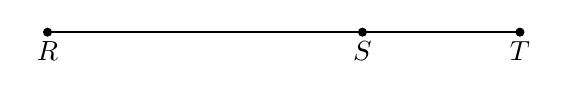
\begin{tikzpicture}
      \draw [-, thick] (1,0)--(7,0);
      \draw [fill] (1,0) circle [radius=0.05] node[below]{$R$};
      \draw [fill] (5,0) circle [radius=0.05] node[below]{$S$};
      \draw [fill] (7,0) circle [radius=0.05] node[below]{$T$};
    \end{tikzpicture}  \vspace{2cm}
  \item The postulate used in this problem is the \rule{6cm}{0.15mm}.
  \end{enumerate}

  \item Given the situation in the diagram, answer each question. Circle True or False. \vspace{0.25cm}
  \begin{multicols}{2}
    \begin{enumerate}
      \item T or F: $\overrightarrow{PU}$ and $\overrightarrow{PT}$ are opposite rays.\bigskip
      \item T or F: $\angle RPT$ and $\angle SPU$ are \\adjacent angles. \bigskip
      \item T or F: $\angle TPU$ is an acute angle.\bigskip

    \end{enumerate}
  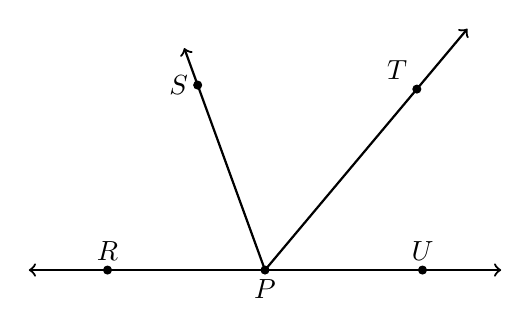
\begin{tikzpicture}[scale=1]
    \draw [->, thick] (0,0)--(50:4);
    \draw [<->, thick] (-3,0)--(3,0);
    \draw [->, thick] (0,0)--(110:3);
    \draw [fill] (110:2.5) circle [radius=0.05] node[left ]{$S$};
    \draw [fill] (50:3) circle [radius=0.05] node[above left ]{$T$};
    \draw [fill] (0,0) circle [radius=0.05] node[below]{$P$};
    \draw [fill] (2,0) circle [radius=0.05] node[above]{$U$};
    \draw [fill] (-2,0) circle [radius=0.05] node[above]{$R$};
  \end{tikzpicture}
  \end{multicols}

  \item Given isosceles $\triangle XYZ$ with $\overline{XY} \cong \overline{YZ}$. On the diagram mark the congruent line segments with tick marks.
  \begin{center}
  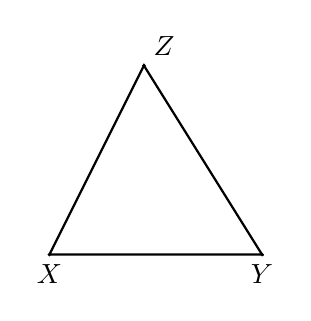
\begin{tikzpicture}[scale=0.3]
    \draw [thick](0,0)--(9,0)--(4,8)--(0,0);
    \draw [fill] (0,0) circle [radius=0.05] node[below]{$X$};
    \draw [fill] (9,0) circle [radius=0.05] node[below]{$Y$};
    \draw [fill] (4,8) circle [radius=0.05] node[above right]{$Z$};
  \end{tikzpicture}
  \end{center}

\end{enumerate}
\end{document}